\chapter{Congruence Subgroups \& Modular Curves}
  Every holomorphic or Maass form is a special type of function depending on certain subgroups of $\PSL_{2}(\Z)$. These are the congruence subgroups. The associated modular curve is the quotient of the upper half-space $\H$ by an action of this subgroup. We introduce these topics first as they are the foundation for discussing holomorphic and Maass forms in complete generality.
  \section{Congruence Subgroups}
    The \textbf{modular group}\index{modular group} is $\PSL_{2}(\Z) = \SL_{2}(\Z)/\{\pm I\}$. That is, the modular group is the set of matrices with integer entries and of determinant $1$ determined up to sign. The reason we are only interested in these matrices up to sign is because the modular group has a natural action on the upper half-space $\H$ and this action will be invariant under a change in sign. The first result usually proved about the modular group is that it is generated by two matrices:

    \begin{proposition}\label{prop:PSL_generator}
        \[
          \PSL_{2}(\Z) = \left\<\begin{pmatrix} 0 &-1 \\ 1 & 0 \end{pmatrix},\begin{pmatrix} 1 & 1 \\ 0 & 1 \end{pmatrix} \right\>.
        \]
    \end{proposition}
    \begin{proof}
      Set $S$ and $T$ to be the first and second generators respectively. Clearly they belong to $\PSL_{2}(\Z)$. Also, $S$ and $T^{n}$ for $n \in \Z$ acts on $\g = \begin{psmallmatrix} a & b \\ c & d \end{psmallmatrix} \in \PSL_{2}(\Z)$ by
      \[
        S\g = S\begin{pmatrix} a & b \\ c & d \end{pmatrix} = \begin{pmatrix} -c & -d \\ a & b \end{pmatrix} \quad \text{and} \quad T^{n}\g = T^{n}\begin{pmatrix} a & b \\ c & d \end{pmatrix} = \begin{pmatrix} a+nc & b+nd \\ c & d \end{pmatrix}.
      \]
      In particular, $S$ interchanges the upper-left and lower-left entries of $\g$ up to sign and $T^{n}$ adds an $n$ multiple of the lower-left entry to the upper-left entry. We have to show $\g \in \<S,T\>$ and we will accomplish this by showing that the inverse is in $\<S,T\>$. If $|c| = 0$ then $\g$ is the identity since $\det(\g) = 1$ so suppose $|c| \neq 0$. By Euclidean division we can write $a = qc+r$ for some $q \in \Z$ and $|r| < |c|$. Then
      \[
        T^{-q}\g = \begin{pmatrix} a-qc & b-qd \\ c & d \end{pmatrix} = \begin{pmatrix} r & b-qd \\ c & d \end{pmatrix}.
      \]
      Multiplying by $S$ yields
      \[
        ST^{-q}\g = S\begin{pmatrix} r & b-qd \\ c & d \end{pmatrix} = \begin{pmatrix} -c & -d \\ r & b-qd \end{pmatrix},
      \]
      and this matrix has the upper-left entry at least as large as the lower-left entry in norm. Actually the upper-left entry is strictly larger since $|c| > |r|$ by Euclidean division. Therefore if we repeatedly apply this procedure, it must terminate with the lower-left entry vanishing. But then we have reached the identity matrix. Therefore we have show $\g$ has an inverse in $\<S,T\>$.
    \end{proof}

    We will also be interested in special subgroups of the modular group defined by congruence conditions on their entries. For $N \ge 1$, set
    \[
      \G(N) = \left\{\begin{pmatrix} a & b \\ c & d \end{pmatrix} \in \PSL_{2}(\Z):\begin{pmatrix} a & b \\ c & d \end{pmatrix} \equiv \begin{pmatrix} 1 & 0 \\ 0 & 1 \end{pmatrix} \tmod{N}\right\}.
    \]
    Then $\G(N)$ is the kernel of the homomorphism $\PSL_{2}(\Z) \to \PSL_{2}(\Z/N\Z)$ given by reducing the coefficients modulo $N$ so it is a normal subgroup with finite index. We call $\G(N)$ the \textbf{principal congruence subgroup}\index{principal congruence subgroup} of level $N$. For $\G \le \PSL_{2}(\Z)$, we say $\G$ is a \textbf{congruence subgroup}\index{congruence subgroup} if $\G(N) \le \G$ for some $N$ and the minimal such $N$ is called the \textbf{level}\index{level} of $\G$. Note that if $M \mid N$, then $\G(N) \le \G(M)$. Thus if $\G$ is a congruence subgroup of level $N$, then $\G(kN) \le \G$ for all $k \ge 1$. This implies that congruence subgroups are closed under intersection. Also, it turns out that the aforementioned homomorphism is surjective:

    \begin{proposition}\label{prop:surjective_modulo_N_for_modular_group}
      The homomorphism $\PSL_{2}(\Z) \to \PSL_{2}(\Z/N\Z)$ given by reducing the coefficients modulo $N$ is surjective.
    \end{proposition}
    \begin{proof}
      Suppose $\begin{psmallmatrix} \conj{a} & \conj{b} \\ \conj{c} & \conj{d} \end{psmallmatrix} \in \SL_{2}(\Z/N\Z)$. Then $\conj{a}\conj{d}-\conj{b}\conj{c} \equiv 1 \tmod{N}$ so by B\'ezout's identity (generalized to three integers) $(\conj{c},\conj{d},N) = 1$. We claim that there exists $s$ and $t$ such that $c = \conj{c}+sN$, $d = \conj{d}+tN$ with $(c,d) = 1$. Set $g = (\conj{c},\conj{d})$. Then $(g,N) = 1$ because $(\conj{c},\conj{d},N) = 1$. If $\conj{c} = 0$ then set $s = 0$ so $c = 0$ and choose $t$ such that $t \equiv 1 \tmod{p}$ for any prime $p \mid g$ and $t \equiv 0 \tmod{p}$ for any prime $p \nmid g$ and $p \mid \conj{d}$. Such a $t$ exists by the Chinese remainder theorem. Now if $p \mid (c,d)$, then either $p \mid g$ or $p \nmid g$. If $p \mid g$, then $p \mid d-\conj{d} = tN$ which is absurd since $t \equiv 1 \tmod{p}$ and $(t,N) = 1$. If $p \nmid g$, then $p \nmid d-\conj{d} = tN$ but this is also absurd since $t \equiv 0 \tmod{p}$. Therefore $(c,d) = 1$ as claimed. If $\conj{c} = 0$ then $\conj{d} \neq 0$, and we can proceed similarly. Since $(c,d) = 1$ there exists $a$ and $b$ such that $ad-bc = 1$. Then $\begin{psmallmatrix} a & b \\ c & d \end{psmallmatrix} \in \PSL_{2}(\Z)$ and maps onto $\begin{psmallmatrix} \conj{a} & \conj{b} \\ \conj{c} & \conj{d} \end{psmallmatrix}$. This proves surjectivity.
    \end{proof}
    
      By \cref{prop:surjective_modulo_N_for_modular_group}, $[\PSL_{2}(Z):\G(N)] = |\PSL_{2}(\Z/N\Z)|$. Since $\G(N) \le \G$ and $\G(N)$ has finite index in $\PSL_{2}(\Z)$ so does $\G$. The subgroups
    \[
      \G_{1}(N) = \left\{\begin{pmatrix} a & b \\ c & d \end{pmatrix} \in \PSL_{2}(\Z):\begin{pmatrix} a & b \\ c & d \end{pmatrix} \equiv \begin{pmatrix} 1 & \ast \\ 0 & 1 \end{pmatrix} \tmod{N}\right\},
    \]
    and
    \[
      \G_{0}(N) = \left\{\begin{pmatrix} a & b \\ c & d \end{pmatrix} \in \PSL_{2}(\Z):\begin{pmatrix} a & b \\ c & d \end{pmatrix} \equiv \begin{pmatrix} \ast & \ast \\ 0 & \ast \end{pmatrix} \tmod{N}\right\},
    \]
    are particularly important and are congruence subgroups of level $N$. The latter subgroup is called the \textbf{Hecke congruence subgroup}\index{Hecke congruence subgroup} of level $N$. Note that $\G(N) \le \G_{1}(N) \le \G_{0}(N)$. If $\G$ is a general congruence subgroup, it is useful to find a generating set for $\G$ in order to reduce results about $\G$ to that of the generators. This is usually achieved by performing some sort of Euclidean division argument on the entries of a matrix $\g \in \G$ using the supposed generating set to construct the inverse for $\g$. We will also require a useful lemma which says that congruence subgroups are preserved under conjugation by elements of $\GL_{2}^{+}(\Q)$ provided we restrict to those elements in $\PSL_{2}(\Z)$:

  \begin{lemma}\label{lem:coset_lemma_1}
    Let $\G$ be a congruence subgroup and let $\a \in \GL_{2}^{+}(\Q)$. Then $\a^{-1}\G\a \cap \PSL_{2}(\Z)$ is a congruence subgroup.
  \end{lemma}
  \begin{proof}
    Recall that if $\G$ is of level $M$, then $\G(kM) \le \G$ for every $k \ge 1$. Thus there is an integer $\wtilde{N}$ such that $\G(\wtilde{N}) \le \G$, $\wtilde{N}\a \in \GL_{2}^{+}(\Z)$, and $\wtilde{N}\a \in \GL_{2}^{+}(\Z)$. Now let $N = \wtilde{N}^{3}$ and notice that any $\g \in \G(N)$ is of the form
    \[
      \g = \begin{pmatrix} 1 & 0 \\ 0 & 1 \end{pmatrix}+N\begin{pmatrix} k_{1} & k_{2} \\ k_{3} & k_{4} \end{pmatrix},
    \]
    for $k_{1},\ldots,k_{4} \in \Z$. Therefore $\G(N) \subseteq I+N\Mat_{2}(\Z)$. Thus
    \[
      \a\G(N)\a^{-1} \le \a(I+N\Mat_{2}(\Z))\a^{-1} = I+\wtilde{N}\Mat_{2}(\Z).
    \]
    As every matrix in $\a\G(N)\a^{-1}$ has determinant $1$ and $\G(\wtilde{N}) \subseteq I+\wtilde{N}\Mat_{2}(\Z)$, it follows that $\a\G(N)\a^{-1} \le \G(\wtilde{N})$. As $\G(\wtilde{N}) \le \G$, we conclude
    \[
      \G(N) \le \a^{-1}\G\a,
    \]
    and intersecting with $\PSL_{2}(\Z)$ completes the proof.
  \end{proof}

  Note that by \cref{lem:coset_lemma_1}, if $\a^{-1}\G\a \subset \PSL_{2}(\Z)$ then $\a^{-1}\G\a$ is a congruence subgroup if $\G$ is. Moreover, since congruence subgroups are closed under intersection, \cref{lem:coset_lemma_1} further implies that $\a^{-1}\G_{1}\a \cap \G_{2}$ is a congruence subgroup for and two congruence subgroups $\G_{1}$ and $\G_{2}$ any any $\a \in \GL_{2}^{+}(\Q)$.
  \section{Modular Curves}
    Recall that $\GL_{2}^{+}(\Q)$ naturally acts on the Riemann sphere $\hat{\C}$ by M\"obius transformations. Explicitly, any $\g = \begin{psmallmatrix} a & b \\ c & d \end{psmallmatrix} \in \GL_{2}^{+}(\Q)$ acts on $z \in \hat{\C}$ by
    \[
      \g z = \frac{az+b}{cz+d},
    \]
    where $\g \infty = \frac{a}{c}$ and $\g\left(-\frac{d}{c}\right) = \infty$. Moreover, recall that this action is a group action, is invariant under scalar multiplication, and acts as automorphisms of $\hat{\C}$. Now observe
    \[
      \Im(\g z) = \Im\left(\frac{az+b}{cz+d}\right) = \Im\left(\frac{az+b}{cz+d}\frac{c\conj{z}+d}{c\conj{z}+d}\right) = \Im\left(\frac{ac|z|^{2}+adz+bc\conj{z}+bd}{|cz+d|^{2}}\right) = \det(\g)\frac{\Im(z)}{|cz+d|^{2}},
    \]
    where the last equality follows because $\Im(\conj{z}) = -\Im(z)$ and $\det(\g) = ad-bc$. Since $\deg(\g) > 0$ and $|cz+d|^{2} > 0$, $\g$ preserves the sign of the imaginary part of $z$. So $\g$ preserves the upper half-space $\H$, the lower half-space $\conj{\H}$, and the extended real line $\hat{\R}$ respectively. Moreover, $\g$ restricts to an automorphism on these subspaces since M\"obius transformations are automorphisms. In particular, $\PSL_{2}(\Z)$ naturally acts on $\hat{\C}$ by M\"obius transformations and preserves the upper half-space. Certain actions of subgroups of $\PSL_{2}(\Z)$ also play important roles. A \textbf{Fuchsian group}\index{Fuchsian group} is any discrete subgroup of $\PSL_{2}(\R)$ that acts properly discontinuously on $\H$ (see \cref{append:Fundamental_Domains}). It turns out that the modular group is a Fuchsian group (see \cite{diamond2005first} for a proof):

    \begin{proposition}\label{prop:modular_group_is_Fuchsian}
      The modular group is a Fuchsian group.
    \end{proposition}

    Note that \cref{prop:modular_group_is_Fuchsian} immediately implies that any subgroup of the modular group is also Fuchsian. In particular, all congruence subgroups are Fuchsian. A \textbf{modular curve}\index{modular curve} is a quotient $\GH$ of the upper half-space $\H$ by the action of a congruence subgroup $\G$. Since $\G$ is Fuchsian and acts on $\H$ by automorphisms \cref{prop:quotient_by_discrete_property_discontinuously} implies that $\GH$ is also connected Hausdorff (recall that $\H$ is connected Hausdorff). In particular, $\GH$ admits the fundamental domain
    \[
      \mc{F} = \left\{z \in \H:\text{$|\Re(z)| \le \frac{1}{2}$ and $|z| \ge 1$}\right\},
    \]
    as the following proposition shows:

    \begin{proposition}\label{prop:fundamental_domain_modular_group}
      $\mc{F}$ is a fundamental domain for $\PSL_{2}(\Z)$.
    \end{proposition}
    \begin{proof}
      Set $\PSL_{2}(\Z) = \<S,T\>$ where $S$ and $T$ are as in \cref{prop:PSL_generator}. We first show any point in $\H$ is $\PSL_{2}(\Z)$-equivalent to a point in $\mc{F}$. Then for any $\g = \begin{psmallmatrix} a & b \\ c & d \end{psmallmatrix} \in \PSL_{2}(\Z)$, we have
      \[
        \Im(\g z) = \frac{\Im(z)}{|cz+d|^{2}} = \frac{y}{(cx+d)^{2}+(cy)^{2}}.
      \]
      Since $\det(\g) = 1$ we cannot have $c = d = 0$. Then as $y \neq 0$, $|cz+d|^{2}$ is bounded away from zero and moreover there are finitely many pairs $(c,d)$ such that $|cz+d|^{2}$ is less than any given upper bound. Therefore there exists $\g_{0} \in \PSL_{2}(\Z)$ that minimizes $|cz+d|^{2}$ and hence maximizes $\Im(\g_{0}z)$. In particular,
      \[
        \Im(S\g_{0}z) = \frac{\Im(\g_{0}z)}{|\g_{0}z|^{2}} \le \Im(\g_{0}z).
      \]
      The inequality above implies $|\g_{0}z| \ge 1$. Since $\Im(T^{n}\g_{0}z) = \Im(\g_{0}z)$ for all $n \in \Z$, repeating the argument above with $T^{n}\g_{0}$ in place of $\g_{0}$, we see that $|T^{n}\g_{0}z| \ge 1$. But $T$ shifts the real part by $1$ so we can choose $n$ such that $|\Re(T^{n}\g_{0}z)| \le \frac{1}{2}$. Therefore $T^{n}\g_{0} \in \PSL_{2}(\Z)$ sends $z$ into $\mc{F}$ as desired. We will now show that if two points in $\mc{F}$ are $\PSL_{2}(\Z)$-equivalent via a non-identity element, then they lie on the boundary of $\mc{F}$. Since $\PSL_{2}(\Z)$ acts on $\H$ by automorphisms, by \cref{prop:PSL_generator} it suffices to show that $S$ and $T$ map $\mc{F}$ outside of $\mc{F}$ except for possibly the boundary. This is clear for $T$ since it maps the left boundary line $\left\{z \in \H:\text{$\Re(z) = -\frac{1}{2}$ and $|z| \ge 1$}\right\}$ to the right boundary line $\left\{z \in \H:\text{$\Re(z) = \frac{1}{2}$ and $|z| \ge 1$}\right\}$ and every other point of $\mc{F}$ is mapped to the right of this line. For $S$, note that it maps the semicircle $\{z \in \H:|z| = 1\}$ to itself (although not identically) and maps $\infty$ to zero. Since M\"obius transformations send circles to circles and lines to lines it follows that every other point of $\mc{F}$ is taken to a point enclosed by the semicircle $\{z \in \H:|z| = 1\}$. Lastly, the interior of $\mc{F}$ is a domain since it is open and path-connected. This finishes the proof.
    \end{proof}

    \begin{figure}[ht]
      \centering
      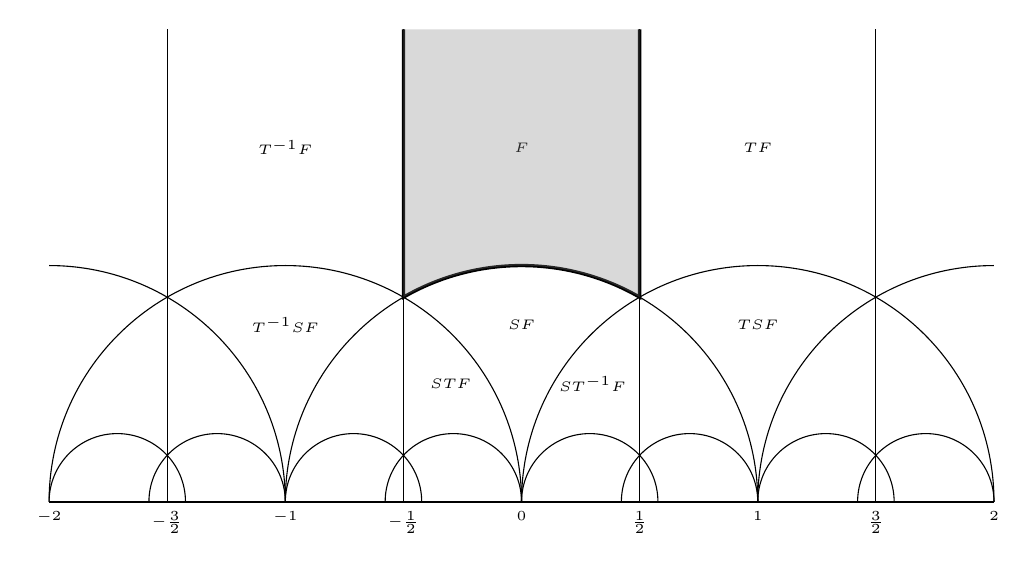
\begin{tikzpicture}[scale=3]
        \def\xmin{-2} \def\xmax{2}
        \def\ymin{0} \def\ymax{2}
        \draw[thick] (\xmin,0) -- (\xmax,0);

        \draw[very thick] (0.5,\ymax) -- (0.5,{sqrt(3)/2}) arc (60:120:1) -- (-0.5,\ymax);

        \node at (-0.5,0) [below] {\tiny{$-\frac{1}{2}$}};
        \node at (0.5,0) [below] {\tiny{$\frac{1}{2}$}};
        \node at (-1.5,0) [below] {\tiny{$-\frac{3}{2}$}};
        \node at (1.5,0) [below] {\tiny{$\frac{3}{2}$}};
        \node at (0,0) [below] {\tiny{$0$}};
        \node at (-1,0) [below] {\tiny{$-1$}};
        \node at (1,0) [below] {\tiny{$1$}};
        \node at (-2,0) [below] {\tiny{$-2$}};
        \node at (2,0) [below] {\tiny{$2$}};

        \draw[thin] (0.5,0) -- (0.5,\ymax);
        \draw[thin] (-0.5,0) -- (-0.5,\ymax);
        \draw[thin] (1.5,0) -- (1.5,\ymax);
        \draw[thin] (-1.5,0) -- (-1.5,\ymax);

        \draw (1,0) arc (0:180:1);
        \draw (-1,0) arc (0:90:1);
        \draw (2,1) arc (90:180:1);

        \draw (0,0) arc (0:180:1);
        \draw (2,0) arc (0:180:1);

        \draw (1,0) arc (0:180:{sqrt(3)/6});
        \draw ({sqrt(3)/3},0) arc (0:180:{sqrt(3)/6});

        \draw (2,0) arc (0:180:{sqrt(3)/6});
        \draw ({1+sqrt(3)/3},0) arc (0:180:{sqrt(3)/6});

        \draw (0,0) arc (0:180:{sqrt(3)/6});
        \draw ({(sqrt(3)/3)-1},0) arc (0:180:{sqrt(3)/6});

        \draw (-1,0) arc (0:180:{sqrt(3)/6});
        \draw ({(sqrt(3)/3)-2},0) arc (0:180:{sqrt(3)/6});

        \node at (0,1.5) {\tiny{$\mc{F}$}};
        \node at (-1,1.5) {\tiny{$T^{-1}\mc{F}$}};
        \node at (1,1.5) {\tiny{$T\mc{F}$}};
        \node at (0,0.75) {\tiny{$S\mc{F}$}};
        \node at (-1,0.75) {\tiny{$T^{-1}S\mc{F}$}};
        \node at (1,0.75) {\tiny{$TS\mc{F}$}};
        \node at (-0.3,0.5) {\tiny{$ST\mc{F}$}};
        \node at (0.3,0.5) {\tiny{$ST^{-1}\mc{F}$}};

        \begin{scope}
          \path[clip] (0.5,\ymax) -- (0.5,{sqrt(3)/2}) arc (60:120:1) -- (-0.5,\ymax) -- cycle;
          \fill[gray,opacity=0.3] (-0.5,0) rectangle (0.5,\ymax);
        \end{scope}
      \end{tikzpicture}
      \caption{The standard fundamental domain for $\PSL_{2}(\Z)\backslash\H$.} \label{fig:fundamental_domain_modular_group}
    \end{figure}
    
    The region $\mc{F}$, shaded in \cref{fig:fundamental_domain_modular_group}, is called the \textbf{standard fundamental domain}\index{standard fundamental domain}. \cref{fig:fundamental_domain_modular_group} also displays how this fundamental domain changes under the actions of the generators of $\PSL_{2}(\Z)$ as in \cref{prop:PSL_generator}. A fundamental domain for any other modular curve can be built from the standard fundamental domain as the following proposition shows (see \cite{kilford2015modular} for a proof):

    \begin{proposition}\label{prop:fundamental_domain_congruence_subgroup}
      Let $\G$ be any congruence subgroup. Then
      \[
        \mc{F}_{\G} = \bigcup_{\g \in \G\backslash\PSL_{2}(\Z)}\g\mc{F},
      \]
      is a fundamental domain for $\G\backslash\H$.
    \end{proposition}

    We might notice that $\mc{F}$ in \cref{fig:fundamental_domain_modular_group} is unbounded as it doesn't contain the point $\infty$. However, if we consider $\mc{F} \cup \{\infty\}$ then it would appear that this space is compact. The point $\infty$ is an example of a cusp and we now make this idea precise. Since any $\g \in \PSL_{2}(\Z)$ preserves $\hat{\R}$ and $\g$ has integer entries, $\g$ also preserves $\Q \cup \{\infty\}$. A \textbf{cusp}\index{cusp} of $\GH$ is an element of of $\G\backslash(\Q \cup \{\infty\})$. As $\G$ has finite index in the modular group, there can only be finitely many cusps and the number of cusps is at most the index of $\G$. In particular, the $\G$-orbit of $\infty$ is a cusp of $\GH$. We denote cusps by gothic characters $\mf{a},\mf{b},\mf{c},\ldots$ or by representatives of their equivalence classes. For example, we let $\infty$ denote the cusp $\G\infty$.

    \begin{remark}
      It turns out that the cusps can be represented as the points needed to make a fundamental domain $\mc{F}_{\G}$ compact as a subset of $\hat{\C}$. To see this, suppose $\mf{a}$ is a limit point of $\mc{F}_{\G}$ that does not belong to $\mc{F}_{\G}$. Then $\mf{a} \in \hat{\R}$. In the case of the standard fundamental domain $\mc{F}$, $\mf{a} = \infty$ which is a cusp. Otherwise, $\mc{F}_{\G}$ is a union of images of $\mc{F}$ by \cref{prop:fundamental_domain_congruence_subgroup} and since $\PSL_{2}(\Z)\infty = \Q \cup \{\infty\}$, we find that $\mf{a} \in \Q \cup \{\infty\}$.
    \end{remark}

    Let $\G_{\mf{a}} \le \G$ denote the stabilizer subgroup of the cusp $\mf{a}$. For the $\infty$ cusp, we can describe $\G_{\infty}$ explicitly. If $\g = \begin{psmallmatrix} a & b \\ c & d \end{psmallmatrix} \in \G$ stabilizes $\infty$, then necessarily $c = 0$ and since $\det(\g) = 1$ we must have $a = d = 1$. Therefore $\g = \begin{psmallmatrix} 1 & b \\ 0 & 1 \end{psmallmatrix}$ for some $b \in \Z$ and $\g$ acts on $\H$ by translation by $b$. Of course, not every translation is guaranteed to belong to $\G$. Letting $t$ be the smallest positive integer such that $\begin{psmallmatrix} 1 & t \\ 0 & 1 \end{psmallmatrix} \in \G$, we have $\G_{\infty} = \left\<\begin{psmallmatrix} 1 & t \\ 0 & 1 \end{psmallmatrix}\right\>$. In particular, $\G_{\infty}$ is an infinite cyclic group. We say that $\G$ is \textbf{reduced at infinity}\index{reduced at infinity} if $t = 1$ so that $\G_{\infty} = \left\<\begin{psmallmatrix} 1 & 1 \\ 0 & 1 \end{psmallmatrix}\right\>$. In particular, $\G_{1}(N)$ and $\G_{0}(N)$ are reduced at infinity.
    
    \begin{remark}
      If $\G$ is of level $N$, then $N$ is the smallest positive integer such that $\G(N) \le \G$ so that $\begin{psmallmatrix} 1 & N \\ 0 & 1 \end{psmallmatrix}$ is the minimal translation guaranteed to belong to $\G$. However, there may be smaller translations so in general $t \le N$.
    \end{remark}
    
    Moreover, for any cusp $\mf{a}$ we have that $\G_{\mf{a}}$ is also an infinite cyclic group and we denote its generator by $\g_{\mf{a}}$. To see this, if $\mf{a} = \frac{a}{c}$ with $(a,c) = 1$ is a cusp of $\GH$ not equivalent to $\infty$, then there exists an $\s_{\mf{a}} \in \PSL_{2}(\Z)$ such that $\s_{\mf{a}}\infty = \mf{a}$. Indeed, there exists integers $d$ and $b$ such that $ad-bc = 1$ by B\'ezout's identity and then $\s_{\mf{a}} = \begin{psmallmatrix} a & b \\ c & d \end{psmallmatrix}$ is such a matrix. It follows that $\G_{\mf{a}} = \s_{\mf{a}}\G_{\infty}\s_{\mf{a}}^{-1}$ and since $\G_{\infty}$ is infinite cyclic so is $\G_{\mf{a}}$. We call any matrix $\s_{\mf{a}} \in \PSL_{2}(\Z)$ satisfying 
    \[
      \s_{\mf{a}}\infty = \mf{a} \quad \text{and} \quad \s_{\mf{a}}^{-1}\g_{\mf{a}}\s_{\mf{a}} = \begin{pmatrix} 1 & t \\ 0 & 1 \end{pmatrix},
    \]
    a \textbf{scaling matrix}\index{scaling matrix} for the cusp $\mf{a}$. Note that $\s_{\mf{a}}$ is determined up to composition on the right by an element of $\G_{\infty}$. Scaling matrices are useful because they allow us to transfer information at the cusp $\mf{a}$ to the cusp at $\infty$. Let $\mf{a}$ and $\mf{b}$ be cusps of $\GH$ with scaling matrices $\s_{\mf{a}}$ and $\s_{\mf{b}}$ respectively. When investigating holomorphic forms, it will be useful to have a double coset decomposition for sets of the form $\s_{\mf{a}}^{-1}\G\s_{\mf{b}}$. This is referred to as the \textbf{Bruhat decomposition}\index{Bruhat decomposition} for $\G$:

    \begin{theorem}[Bruhat decomposition]
      Let $\G$ be any congruence subgroup and let $\mf{a}$ and $\mf{b}$ be cusps of $\GH$ with scaling matrices $\s_{\mf{a}}$ and $\s_{\mf{b}}$ respectively. Then we have the disjoint decomposition
      \[
        \s_{\mf{a}}^{-1}\G\s_{\mf{b}} = \d_{\mf{a},\mf{b}}\W_{\infty}\bigcup_{\substack{c \ge 1 \\ d \tmod{c}}}\W_{d/c},
      \]
      where
      \[
        \W_{\infty} = \G_{\infty}\w_{\infty} = \w_{\infty}\G_{\infty} = \G_{\infty}\w_{\infty}\G_{\infty} \quad \text{and} \quad \W_{d/c} = \G_{\infty}\w_{d/c}\G_{\infty},
      \]
      for some $\w_{\infty} = \begin{psmallmatrix} 1 & \ast \\ 0 & 1 \end{psmallmatrix} \in \s_{\mf{a}}^{-1}\G\s_{\mf{b}}$ and $\w_{d/c} = \begin{psmallmatrix} a & \ast \\ c & d \end{psmallmatrix} \in \s_{\mf{a}}^{-1}\G\s_{\mf{b}}$ with $c \ge 1$ if such a matrix exists otherwise $\W_{d/c}$ is empty. Moreover, the entries $a$ and $d$ of $\w_{d/c}$ are determined modulo $c$.
    \end{theorem}
    \begin{proof}
      We first show that $\W_{\infty}$ is nonempty if and only if $\mf{a} = \mf{b}$. Indeed, if $\w \in \W_{\infty}$ then $\w = \s_{\mf{a}}^{-1}\g\s_{\mf{b}}$ for some $\g \in \G$. Then
      \[
        \g\mf{b} = \s_{\mf{a}}\w\s_{\mf{b}}^{-1}\mf{b} = \s_{\mf{a}}\w\infty = \s_{\mf{a}}\infty = \mf{a}.
      \]
      This shows that $\mf{a} = \mf{b}$. Conversely, suppose $\mf{a} = \mf{b}$. Then $\s_{\mf{a}}^{-1}\G\s_{\mf{b}}$ contains $\s_{\mf{a}}^{-1}\G_{\mf{a}}\s_{\mf{a}} = \G_{\infty}$ so that $\W_{\infty}$ is nonempty. So $\W_{\infty}$ is nonempty if and only if $\mf{a} = \mf{b}$. In this case, for any two elements $\w = \s_{\mf{a}}^{-1}\g\s_{\mf{a}}$ and $\w' = \s_{\mf{a}}^{-1}\g'\s_{\mf{a}}$ of $\W_{\infty}$, we have
      \[
        \g'\g^{-1}\mf{a} = \s_{\mf{a}}\w'\w^{-1}\s_{\mf{a}}^{-1}\mf{a} = \s_{\mf{a}}\w'\w^{-1}\infty = \s_{\mf{a}}\mf{a}.
      \]
      Hence $\g'\g^{-1} \in \G_{\mf{a}}$ which implies $\w'\w^{-1} = \s_{\mf{a}}^{-1}\g'\g^{-1}\s_{\mf{a}} \in \s_{\mf{a}}^{-1}\G_{\mf{a}}\s_{\mf{a}} = \G_{\infty}$. Therefore
      \[
        \W_{\infty} = \G_{\infty}\w = \w\G_{\infty} = \G_{\infty}\w\G_{\infty},
      \]
      where the latter two equalities hold because $\w$ is a translation and translations commute. Every other element of $\s_{\mf{a}}^{-1}\G\s_{\mf{b}}$ belongs to one of the double cosets $\W_{d/c}$ with $c \ge 1$ (since we are working in $\PSL_{2}(\Z)$). The relation
      \[
        \begin{pmatrix} 1 & n \\ 0 & 1 \end{pmatrix}\begin{pmatrix} a & \ast \\ c & d \end{pmatrix}\begin{pmatrix} 1 & m \\ 0 & 1 \end{pmatrix} = \begin{pmatrix} a+cn & \ast \\ c & d+cm \end{pmatrix},
      \]
      shows that $\W_{d/c}$ is determined uniquely by $c$ and $d \tmod{c}$. Moreover, this relation shows that $a$ and $d$ are determined modulo $c$. This completes the proof of the theorem.
    \end{proof}

    Notice that the Bruhat decomposition for $\s_{\mf{a}}^{-1}\G\s_{\mf{b}}$ implies
    \[
      \G_{\infty}\backslash\s_{\mf{a}}^{-1}\G\s_{\mf{b}} = \d_{\mf{a},\mf{b}}\w_{\infty}\bigcup_{\substack{c \ge 1 \\ d \tmod{c}}}\w_{d/c}\G_{\infty},
    \]
    where it is understood that the coset $\w_{d/c}\G_{\infty}$ is empty if the double coset $\W_{d/c}$ is too. This shows that every element of $\G_{\infty}\backslash\s_{\mf{a}}^{-1}\G\s_{\mf{b}}$ corresponds to a unique $(c,d) \in \Z^{2}-\{\mathbf{0}\}$ with $c \ge 1$, $d \in \Z$, and $(c,d) = 1$, and additionally the pair $(0,1)$ if and only if $\mf{a} = \mf{b}$ (this pair corresponds to $\w_{\infty}$). Of course, this correspondence need not be surjective since many of the double cosets $\W_{d/c}$ may be empty. To track such $c$ and $d$ for which $\W_{d/c}$ is nonempty, let $\mc{C}_{\mf{a},\mf{b}}$ and $\mc{D}_{\mf{a},\mf{b}}(c)$ be the sets given by
    \[
      \mc{C}_{\mf{a},\mf{b}} = \left\{c \ge 1: \begin{pmatrix} \ast & \ast \\ c & \ast \end{pmatrix} \in \s_{\mf{a}}^{-1}\G\s_{\mf{b}}\right\} \quad \text{and} \quad \mc{D}_{\mf{a},\mf{b}}(c) = \left\{d \tmod{c}: \begin{pmatrix} \ast & \ast \\ c & d \end{pmatrix} \in \s_{\mf{a}}^{-1}\G\s_{\mf{b}}\right\}.
    \]
    Then $\mc{C}_{\mf{a},\mf{b}}$ and $\mc{D}_{\mf{a},\mf{b}}(c)$ are precisely the sets of $c$ and $d$ take modulo $c$ such that $\W_{d/c}$ is nonempty.

    \begin{remark}\label{rem:Bruhat_modulo_infity_exact}
      The Bruhat decomposition for $\s_{\mf{a}}^{-1}\G\s_{\mf{b}}$ implies
      \[
        \G_{\infty}\backslash\s_{\mf{a}}^{-1}\G\s_{\mf{b}} = \d_{\mf{a},\mf{b}}\w_{\infty}\bigcup_{\substack{c \in \mc{C}_{\mf{a},\mf{b}} \\ d \in \mc{D}_{\mf{a},\mf{b}}(c)}}\w_{d/c}\G_{\infty},
      \]
      where none of the cosets $\w_{d/c}\G_{\infty}$ are empty. In particular, $\g = \begin{psmallmatrix} \ast & \ast \\ c & d \end{psmallmatrix} \in \G_{\infty}\backslash\s_{\mf{a}}^{-1}\G\s_{\mf{b}}$ if and only if $(c,d)$ is a pair with $c \in \mc{C}_{\mf{a},\mf{b}}$, $d \in \Z$, and $d \tmod{c} \in \mc{D}_{\mf{a},\mf{b}}(c)$, or additionally $(0,1)$ if $\mf{a} = \mf{b}$.
    \end{remark}
    
    We will now introduce Kloosterman \& Sali\'e sums associated to cusps. We being with the Kloosterman sums. Let $\s_{\mf{a}}$ and $\s_{\mf{b}}$ be scaling matrices for the cusps $\mf{a}$ and $\mf{b}$ respectively. Then for any $c \in \mc{C}_{\mf{a},\mf{b}}$ and $n,m \in \Z$, the \textbf{generalized Kloosterman sum}\index{generalized Kloosterman sum} $K_{\mf{a},\mf{b}}(n,m,c)$ relative to $\mf{a}$ and $\mf{b}$ is defined by
    \[
      K_{\mf{a},\mf{b}}(n,m,c) = \sum_{d \in \mc{D}_{\mf{a},\mf{b}}(c)}e^{\frac{2\pi i(an+\conj{a}m)}{c}},
    \]
    where $a$ has been determined by $ad-bc = 1$. This sum is well-defined by the Bruhat decomposition because $a$ is determined modulo $c$. In general, $K_{\mf{a},\mf{b}}(n,m,c)$ is not independent of the scaling matrices $\s_{\mf{a}}$ and $\s_{\mf{b}}$. However, if $n = m = 0$ we trivially see by the Bruhat decomposition for $\G$ that
    \[
      K_{\mf{a},\mf{b}}(0,0,c) = \left|\left\{d \tmod{c}:\begin{pmatrix} \ast & \ast \\ c & d \end{pmatrix} \in \s_{\mf{a}}^{-1}\G\s_{\mf{b}}\right\}\right|,
    \]
    which is independent of the scaling matrices $\s_{\mf{a}}$ and $\s_{\mf{b}}$. Moreover, for $\G = \G_{1}(1)$ we have $\mf{a} = \mf{b} = \infty$ and the Bruhat decomposition for $\G_{1}(1)$ implies
    \[
      K_{\infty,\infty}(n,m,c) = K(n,m,c),
    \]
    is the usual Kloosterman sum. Therefore if $\mf{a} = \mf{b} = \infty$, we will suppress these dependencies accordingly. The Sali\'e sums are defined in a similar manner. Let $\s_{\mf{a}}$ and $\s_{\mf{b}}$ be scaling matrices for the cusps $\mf{a}$ and $\mf{b}$ respectively. Then for any $c \in \mc{C}_{\mf{a},\mf{b}}$, and $n,m \in \Z$, and Dirichlet character $\chi$ with conductor $q \mid c$, the \textbf{generalized Sali\'e sum}\index{generalized Sali\'e sum} $S_{\chi,\mf{a},\mf{b}}(n,m,c)$ relative to $\mf{a}$ and $\mf{b}$ is defined by
    \[
      S_{\chi,\mf{a},\mf{b}}(n,m,c) = \sum_{d \in \mc{D}_{\mf{a},\mf{b}}(c)}\chi(a)e^{\frac{2\pi i(an+\conj{a}m)}{c}},
    \]
    where $a$ has been determined by $ad-bc = 1$. This sum is well-defined by the Bruhat decomposition because $a$ is determined modulo $c$. Like the generalized Kloosterman sum, $S_{\mf{a},\mf{b}}(n,m,c)$ need not independent of the scaling matrices $\s_{\mf{a}}$ and $\s_{\mf{b}}$. Moreover, for $\G = \G_{1}(1)$ we have $\mf{a} = \mf{b} = \infty$ and the Bruhat decomposition for $\G_{1}(1)$ implies
    \[
      S_{\chi,\infty,\infty}(n,m,c) = S_{\chi}(n,m,c),
    \]
    is the usual Sali\'e sum. Therefore if $\mf{a} = \mf{b} = \infty$, we will suppress these dependencies accordingly.
  \section{The Hyperbolic Measure}
    We will also need to integrate over $\GH$. In order to do this, we require a measure on $\H$. Our choice of measure will be the \textbf{hyperbolic measure}\index{hyperbolic measure} $d\mu$ given by
    \[
      d\mu = d\mu(z) = \frac{dx\,dy}{y^{2}}.
    \]
    The most important property about the hyperbolic measure is that it is $\GL_{2}^{+}(\R)$-invariant (see \cite{diamond2005first} for a proof):

    \begin{proposition}
      The hyperbolic measure $d\mu$ is $\GL_{2}^{+}(\R)$-invariant.
    \end{proposition}

    As this fact will be used so frequently any time we integrate, we will not mention it explicitly. A particularly important fact is that if $\G$ is a congruence subgroup then $d\mu$ is $\G$-invariant. One of the reasons this is useful is because we can apply the unfolding/folding method to many integrals. The most common instance is when we are integrating the sum $\sum_{\g \in \GG}f(\g z)$ of some holomorphic function $f(z)$ over a fundamental domain $\mc{F}_{\G}$ for $\GH$. Indeed, $\H = \bigcup_{\g \in \G}\g\mc{F}_{\G}$ and so $\G_{\infty}\backslash\H = \bigcup_{\g \in \GG}\g\mc{F}_{\G}$. Since $\mc{F}_{\G}$ is a fundamental domain, the conditions of the unfolding/folding method are satisfied and it follows that
    \[
      \int_{\mc{F}_{\G}}\sum_{\g \in \GG}f(\g z)\,d\mu = \int_{\G_{\infty}\backslash\H}f(z)\,d\mu,
    \]
    provided either side is absolutely convergent. It is also worth highlighting another fact. Any $\a \in \GL_{2}^{+}(\Q)$ acts as an automorphism of $\H$ which implies that it induces a bijection between $\a^{-1}\G\a\backslash\H$ and $\G\backslash\H$ and hence between the fundamental domains $\mc{F}_{\a^{-1}\G\a}$ and $\mc{F}_{\G}$. Thus the change of variables $z \to \a z$ transforms the fundamental domain $\mc{F}_{\G}$ into $\mc{F}_{\a^{-1}\G\a}$. Therefore
    \[
      \int_{\mc{F}_{\G}}f(z)\,d\mu = \int_{\mc{F}_{\a^{-1}\G\a}}f(\a z)\,d\mu,
    \]
    provided either side is bounded. Now let us discuss the volume of $\GH$. We define the \textbf{volume}\index{volume} $V_{\G}$ of $\GH$ by
    \[
      V_{\G} = \int_{\mc{F}_{\G}}\,d\mu.
    \]
    In other words, $V_{\G}$ is the volume of the fundamental domain $\mc{F}_{\G}$ with respect to the hyperbolic measure. Also, if $\mc{F}_{\G} = \mc{F}$ we write $V_{\G} = V$. Since the integrand is $\G$-invariant, $V_{\G}$ is independent of the choice of fundamental domain. Using \cref{prop:fundamental_domain_modular_group}, we have
    \[
      V = \int_{\mc{F}}\,d\mu = \int_{-\frac{1}{2}}^{\frac{1}{2}}\int_{\sqrt{1-x^{2}}}^{\infty}\frac{dy\,dx}{y^{2}} = \int_{-\frac{1}{2}}^{\frac{1}{2}}\frac{1}{\sqrt{1-x^{2}}}\,dx = \arcsin(x)\bigg|_{-\frac{1}{2}}^{\frac{1}{2}} = \frac{\pi}{3}.
    \]
    Therefore $V$ is finite. There is also a simple relation between $V_{\G}$ and the index of $\G$ in $\PSL_{2}(\Z)$:
    \begin{equation}\label{equ:Petersson_volume_relation}
      V_{\G} = [\PSL_{2}(\Z):\G]V,
    \end{equation}
    which follows immediately from \cref{prop:fundamental_domain_congruence_subgroup}. Moreover, $V_{\G}$ is finite for every congruence subgroup $\G$ by \cref{equ:Petersson_volume_relation} and that congruence subgroups have finite index in the modular group. A particularly nice application of this fact is that any integral of the form
    \[
      \frac{1}{V_{\G}}\int_{\mc{F}_{\G}}f(z)\,d\mu,
    \]
    is absolutely convergent provided $f(z)$ is bounded. That is, bounded functions are absolutely convergent over $\mc{F}_{\G}$ with respect to $d\mu$. Moreover, we have a useful lemma:

    \begin{lemma}\label{lem:invariance_of_volume}
      Let $\G$ be a congruence subgroup and $\a \in \GL_{2}^{+}(\Q)$. If $\a^{-1}\G\a \subseteq \PSL_{2}(\Z)$, then $V_{\a^{-1}\G\a} = V_{\G}$ and $[\PSL_{2}(\Z):\a^{-1}\G\a] = [\PSL_{2}(\Z):\G]$.
    \end{lemma}
    \begin{proof}
      The first statement follows from the chain
      \[
        V_{\a^{-1}\G\a} = \int_{\mc{F}_{\a^{-1}\G\a}}\,d\mu = \int_{\mc{F}_{\G}}\,d\mu = V_{\G},
      \]
      where the middle equality is justified by making the change of variables $z \to \a^{-1}z$. The second statement is now immediate from \cref{equ:Petersson_volume_relation}.
    \end{proof}